\section{Results}
Resulting from the work are the squared l2 distances calculated with the program openface. The distance shows the similiarity to the given subjects. A lower distance means the compared two persons are more equal, when the distance is under a given threshold, these two persons are accepted to be the same person and so access is given. The resulting morphed photos were compared to diffrent photos of both subjects, to get a independend distance. For every morph there were 15 images created from 0\% of Subject 1 to 100\%, respectively the remaining \% of Person 2. So the are images combined of:
\begin{itemize}
\item 1. Picture: Person 1 100\% - Person 2 0\%
\item 2. Picture: Person 1 92,86\% - Person 2 7,14\%
\item 3. Picture: Person 1 85,71\% - Person 2 14,29\%
\item 4. Picture: Person 1 78,57\% - Person 2 21,43\%
\item 5. Picture: Person 1 71,43\% - Person 2 28,57\%
\item 6. Picture: Person 1 64,29\% - Person 2 35,71\%
\item 7. Picture: Person 1 57,14\% - Person 2 42,86\%
\item 8. Picture: Person 1 50,00\% - Person 2 50,00\%
\item 9. Picture: Person 1 42,86\% - Person 2 57,14\%
\item 10. Picture: Person 1 35,71\% - Person 2 64,29\%
\item 11. Picture: Person 1 28,57\% - Person 2 71,43\%
\item 12. Picture: Person 1 21,43\% - Person 2 78,57\%
\item 13. Picture: Person 1 14,29\% - Person 2 85,71\%
\item 14. Picture: Person 1 7,14\% - Person 2 92,86\%
\item 15. Picture: Person 1 0\% - Person 2 100\%
\end{itemize}

\subsection{Distances}
\subsubsection{Subset of 5 morph sets (from subjects also used by Budrhani)}
All resulting squared l2 distances for the morphed photos of subjects 01-m-002-27 to 01-m-003-24, 01-m-003-24 to 01-m-005-23, 01-m-004-23 to 01-m-005-23, 01-m-010-23 to 01-m-013-23 and 01-m-014-23 to 01-m-016-23 compared to the corresponding compare images are way too many data. So there is as an example the morphed photo 01-m-002-27 to 01-m-003-24:

\begin{tabular}{lrrrrrr}
	Picture & 01-m-002-28.jpg & 01-m-002-29.jpg & 01-m-002-30.jpg & 01-m-003-25.jpg & 01-m-003-26.jpg & 01-m-003-27.jpg \\
	 & & & & & & \\
	1 & 0.11916 & 0.07499 & 0.19188 & 1.30874 & 1.16709 & 1.31322\\
	2 & 0.13701 & 0.06885 & 0.18756 & 1.25716 & 1.10248 & 1.25841\\ 
	3 & 0.17384 & 0.06523 & 0.19060 & 1.17656 & 1.01354 & 1.17311\\ 
	4 & 0.22901 & 0.07982 & 0.21253 & 1.08009 & 0.90457 & 1.06856\\ 
	5 & 0.31766 & 0.12439 & 0.24763 & 0.89989 & 0.70834 & 0.88006\\ 
	6 & 0.39700 & 0.16766 & 0.30990 & 0.83492 & 0.62518 & 0.81035\\ 
	7 & 0.50975 & 0.24823 & 0.40167 & 0.72848 & 0.51501 & 0.70676\\ 
	8 & 0.67400 & 0.39087 & 0.53792 & 0.60985 & 0.39251 & 0.59632\\ 
	9 & 0.74737 & 0.46525 & 0.58010 & 0.52552 & 0.32146 & 0.50314\\ 
	10 & 0.94108 & 0.62628 & 0.74969 & 0.40924 & 0.21060 & 0.37129\\ 
	11 & 1.05918 & 0.76321 & 0.86483 & 0.32472 & 0.13804 & 0.28219\\ 
	12 & 1.21209 & 0.90143 & 0.99503 & 0.25177 & 0.08833 & 0.20977\\ 
	13 & 1.25246 & 0.97993 & 1.05583 & 0.19876 & 0.05832 & 0.17236\\ 
	14 & 1.34758 & 1.07654 & 1.14637 & 0.19252 & 0.04679 & 0.16232\\ 
	15 & 1.37122 & 1.13813 & 1.18339 & 0.14941 & 0.05522 & 0.13605\\ 
\end{tabular}\\


Also shown in figure \ref{fig:Result1}.

The results of the 01-m-002-27 to 01-m-003-24, 01-m-003-24 to 01-m-005-23, 01-m-004-23 to 01-m-005-23, 01-m-010-23 to 01-m-013-23 and 01-m-014-23 to 01-m-016-23 morphs are shown in figure \ref{fig:Result1-5}.

For better recognizability the mean value of all the diffrent squared l2 distances is calculated for Person 1 and Person 2. The result is shwon in figure \ref{fig:Result1-5-mean}.

As visible the lowest distance to both persons is at Picture 9 (Person 1 42,86\% - Person 2 57,14\%) wtih a minimal distance of \textbf{0.485}.\\

Openface uses normally a threshold of \textbf{0.99}, which allows nearly all morphs from Picture 5 to 10 to be successfull acknowledged as shown in figure \ref{fig:Result1-5}. Only in 3 cases there is the distance way too high to work properly. The compared photos are 01-m-016-24.jpg, 01-m-016-25.jpg and 01-m-016-26.jpg from the same person, so this morph is not working. As a result in 4 out of 5 cases it is possible to morph two subjects to be successfull acknowledged, this makes a sucess chance of 80\%.

\begin{figure}[htbp] 
	\centering
		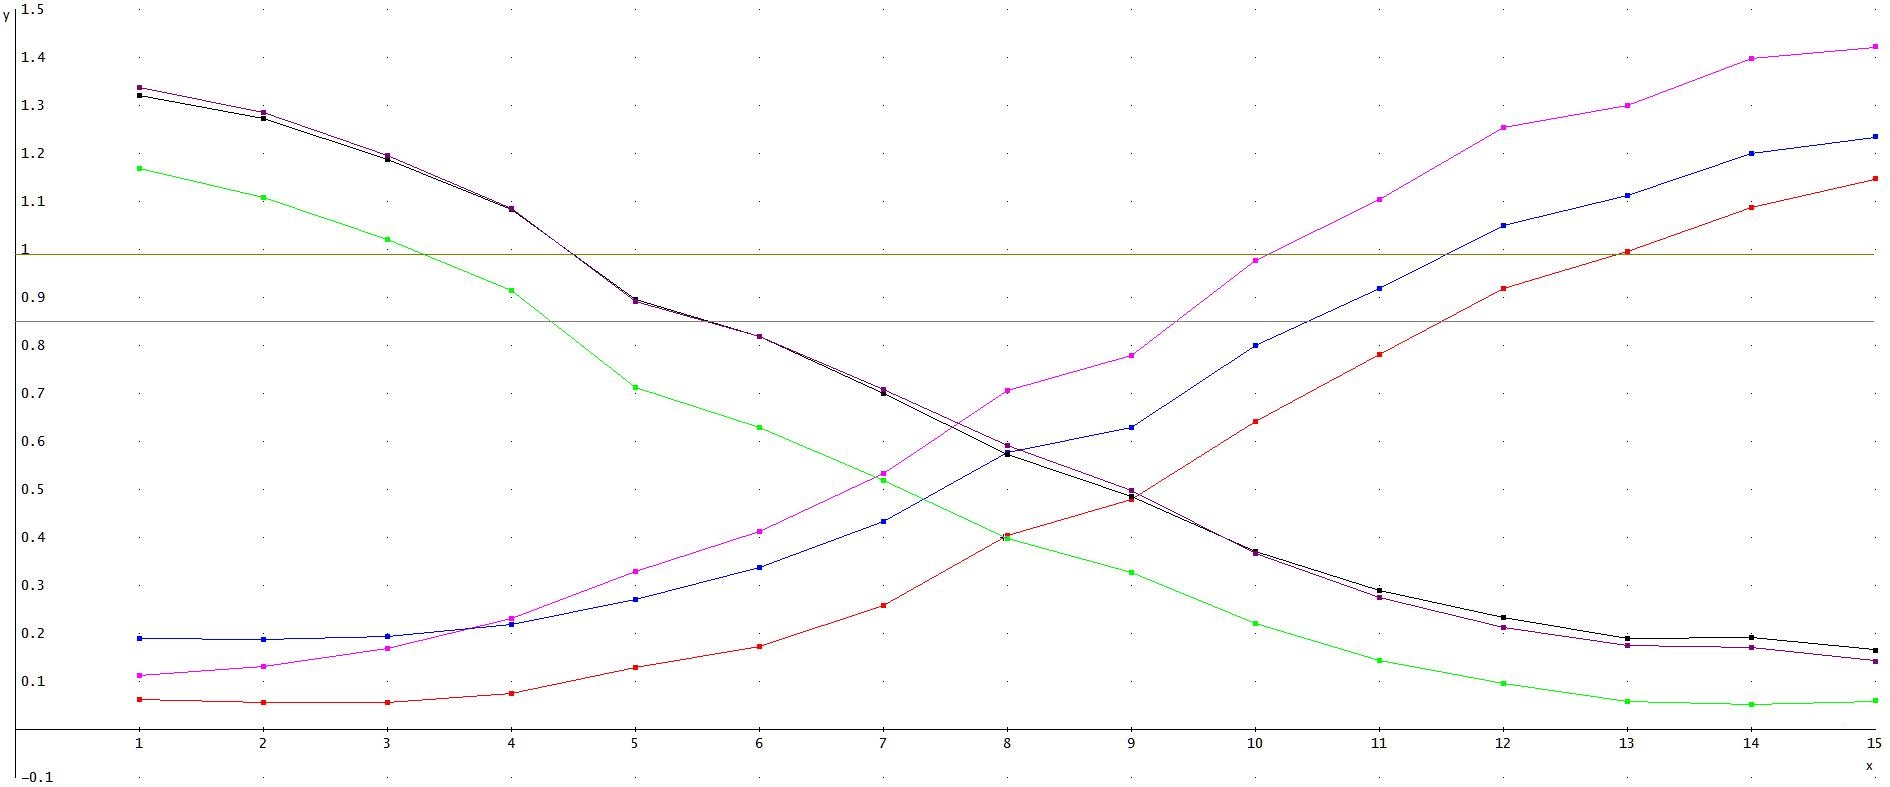
\includegraphics[width=0.95\textwidth]{Resources/result1.jpg}
	\caption{Squared l2 distances (y axis) of morphs from 01-m-002-27 to 01-m-003-24 (with 15 steps ont he x axis) comparing to 01-m-002-28.jpg, 01-m-002-29.jpg, 01-m-002-30.jpg, 01-m-003-25.jpg, 01-m-003-26.jpg and 01-m-003-27.jpg}
	\label{fig:Result1}
\end{figure}

\begin{figure}[htbp] 
	\centering
		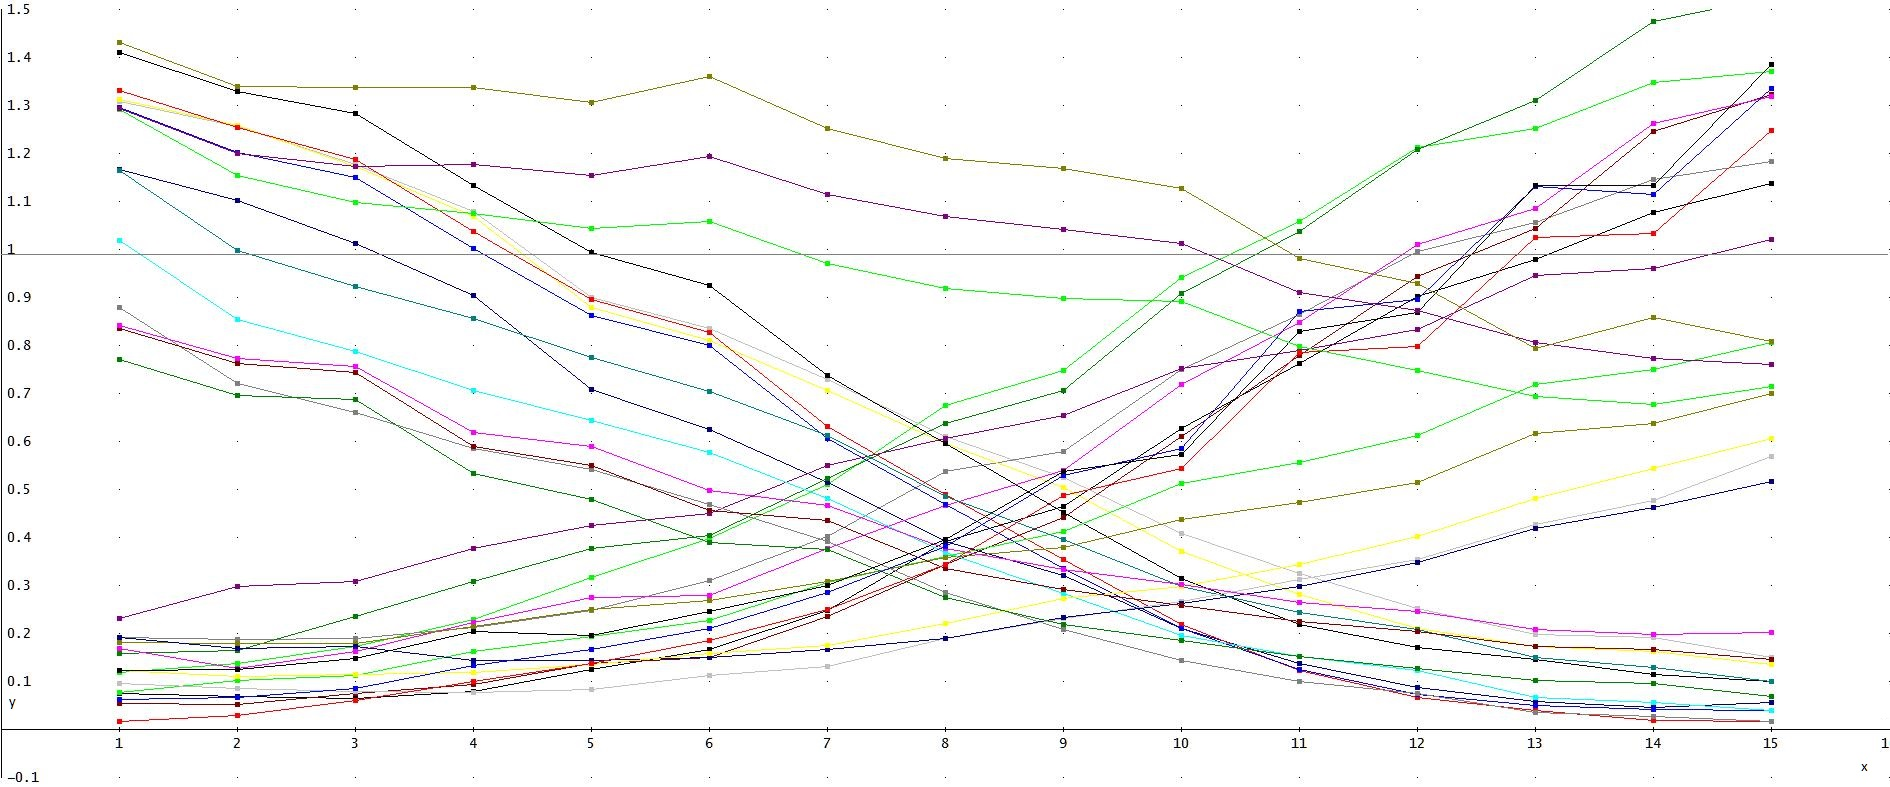
\includegraphics[width=0.95\textwidth]{Resources/result1-5.jpg}
	\caption{Squared l2 distances (y axis) of morphs from 01-m-002-27 to 01-m-003-24, 01-m-003-24 to 01-m-005-23, 01-m-004-23 to 01-m-005-23, 01-m-010-23 to 01-m-013-23 and 01-m-014-23 to 01-m-016-23 (with 15 steps on the x axis) comparing to the corresponding compare photos}
	\label{fig:Result1-5}
\end{figure}

\begin{figure}[htbp] 
	\centering
		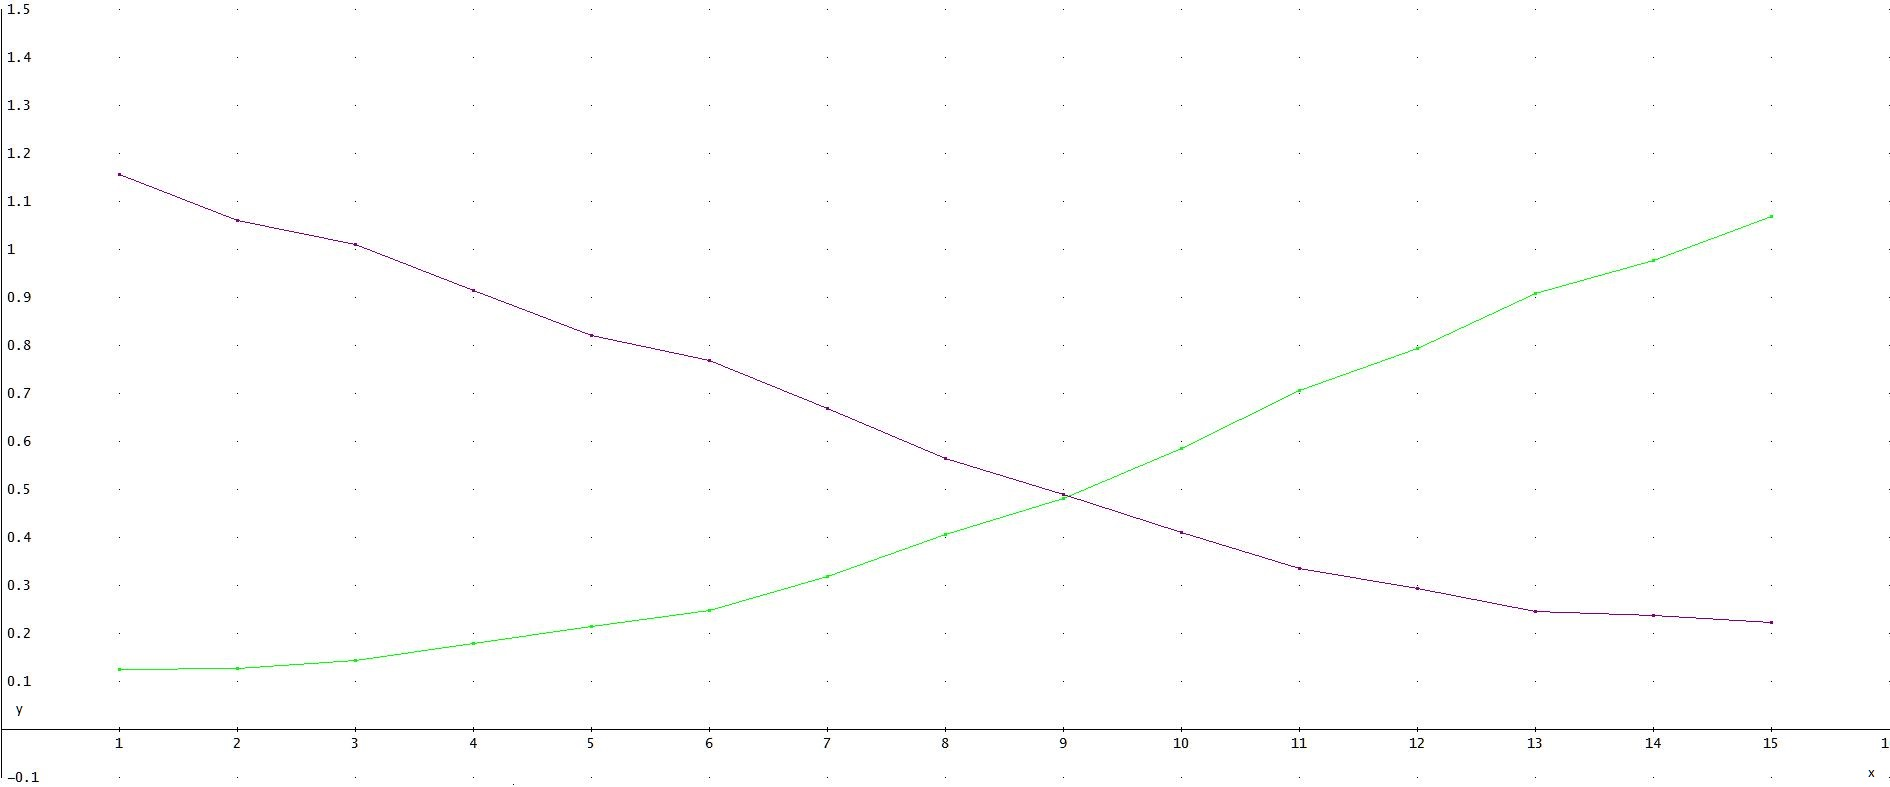
\includegraphics[width=0.95\textwidth]{Resources/result1-5-mean.jpg}
	\caption{Mean squared l2 distances (y axis) of morphs from 01-m-002-27 to 01-m-003-24, 01-m-003-24 to 01-m-005-23, 01-m-004-23 to 01-m-005-23, 01-m-010-23 to 01-m-013-23 and 01-m-014-23 to 01-m-016-23 (with 15 steps on the x axis) comparing to the corresponding compare photos}
	\label{fig:Result1-5-mean}
\end{figure}
\newpage
\subsubsection{Subset of 39 morph sets}\label{sec:subset39}
Now 39 sets of morphed subjects were used. The used subjects are:
\begin{multicols}{3}
\begin{itemize}
\item 01-m-002 - 01-m-003
\item 01-m-003 - 01-m-004
\item 01-m-004 - 01-m-005
\item 01-m-013 - 01-m-014
\item 01-m-016 - 01-m-017
\item 01-m-019 - 01-m-020
\item 01-m-020 - 01-m-021
\item 01-m-021 - 01-m-022
\item 01-m-022 - 01-m-023
\item 01-m-025 - 01-m-026
\item 01-m-026 - 01-m-027
\item 01-m-030 - 01-m-031
\item 01-m-031 - 01-m-032
\item 01-m-032 - 01-m-033
\item 01-m-037 - 01-m-038
\item 01-m-038 - 01-m-039
\item 01-m-039 - 01-m-040
\item 01-m-040 - 01-m-041
\item 01-m-041 - 01-m-042
\item 01-m-042 - 01-m-043
\item 01-m-043 - 01-m-044
\item 01-m-044 - 01-m-045
\item 01-m-045 - 01-m-046
\item 01-m-046 - 01-m-047
\item 01-m-047 - 01-m-048
\item 01-m-048 - 01-m-049
\item 01-m-051 - 01-m-052
\item 01-m-052 - 01-m-053
\item 01-m-053 - 01-m-054
\item 01-m-054 - 01-m-055
\item 01-m-055 - 01-m-056
\item 01-m-059 - 01-m-060
\item 01-m-060 - 01-m-061
\item 01-m-065 - 01-m-066
\item 01-m-066 - 01-m-067
\item 01-m-069 - 01-m-070
\item 01-m-072 - 01-m-073
\item 01-m-073 - 01-m-074
\item 01-m-074 - 01-m-075
\end{itemize}
\end{multicols}


With these sets again the squarred l2 distance is computed to the associated compare images of the two subjects. The resulting distances are shown in figure \ref{fig:Result39-all}. To decrease the amount of information the mean values for both subjects were computed and are shown in figure \ref{fig:Result39-mean}.
\begin{figure}[htbp] 
	\centering
		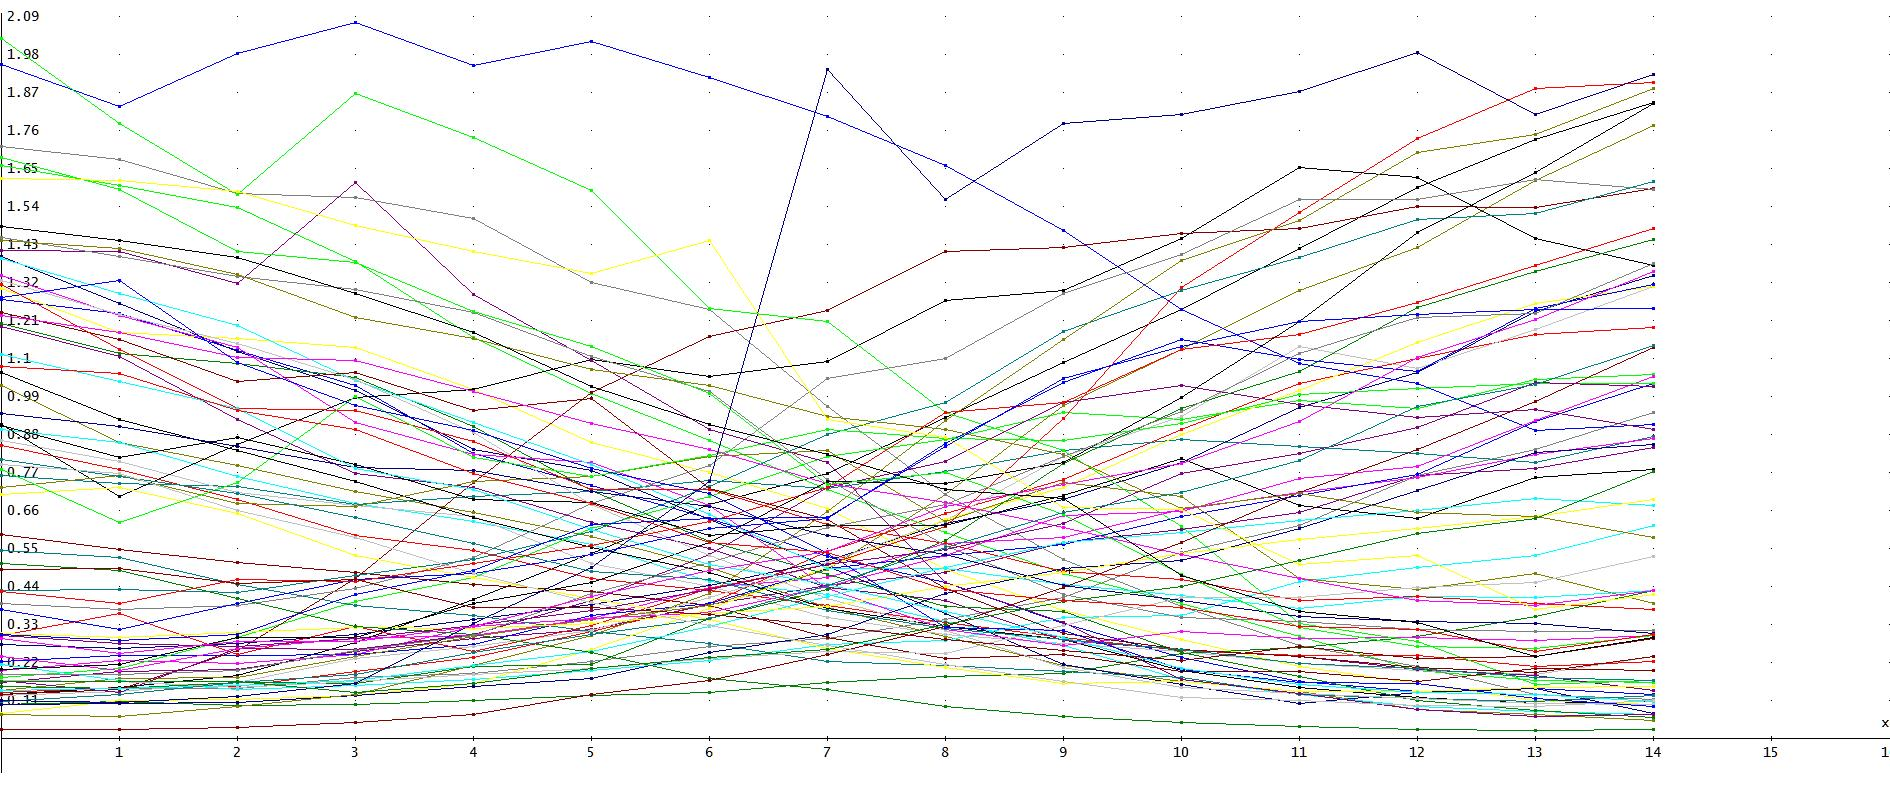
\includegraphics[width=0.95\textwidth]{Resources/result39-all.jpg}
	\caption{Squared l2 distances (y axis) of the subset of 39 morphs (with 15 steps on the x axis) comparing to the corresponding compare photos}
	\label{fig:Result39-all}
\end{figure}
\begin{figure}[htbp] 
	\centering
		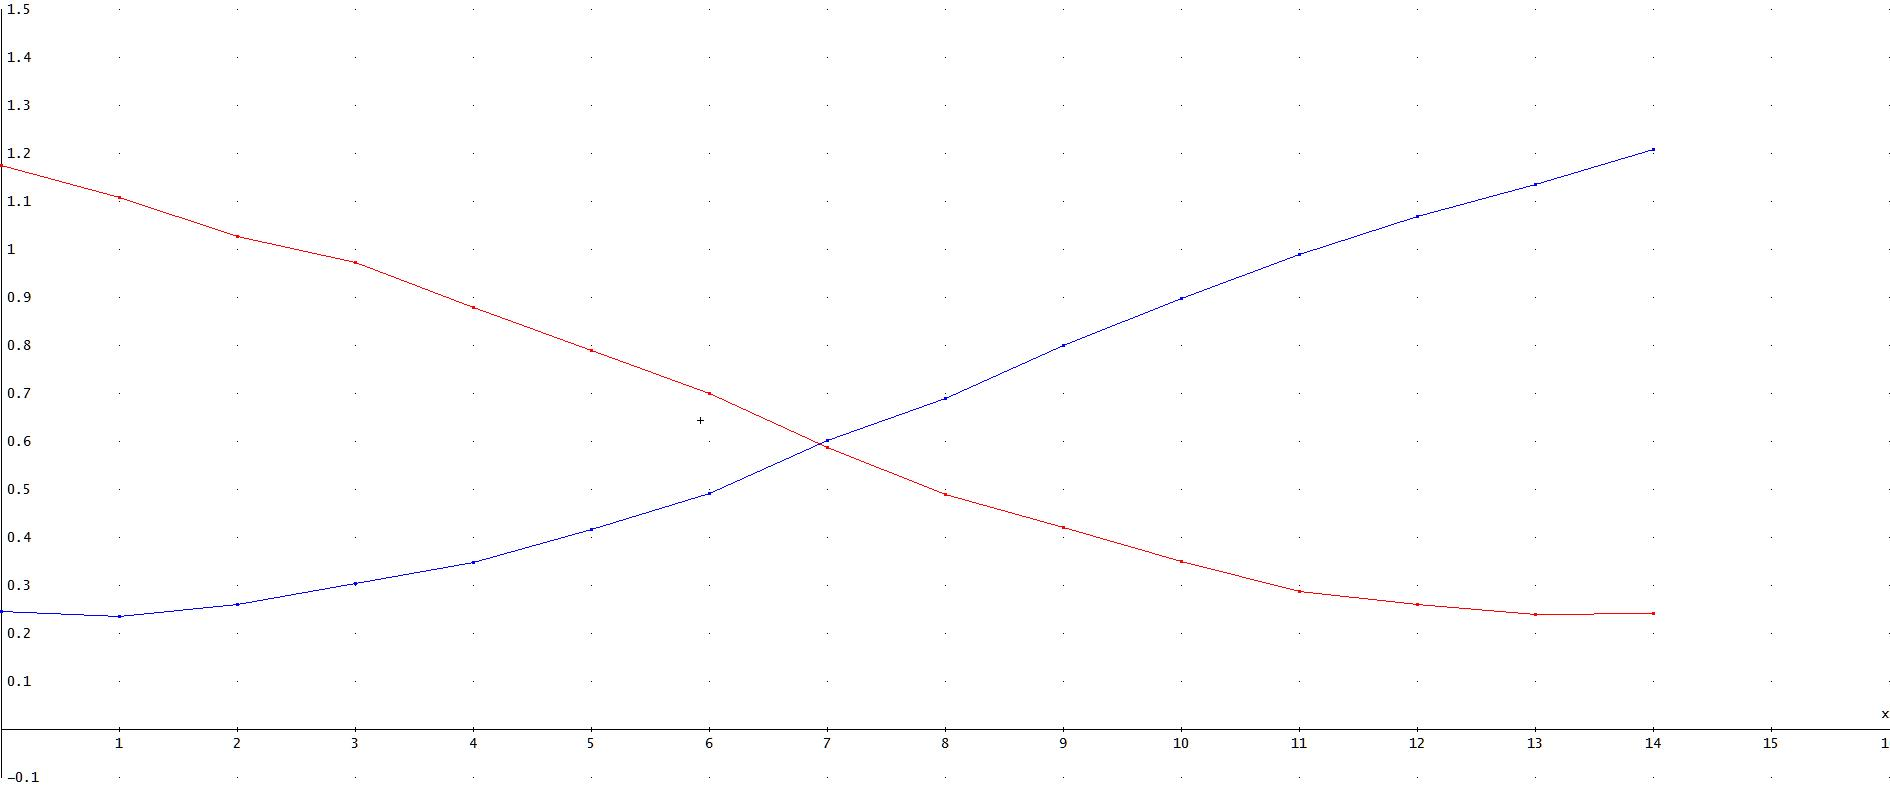
\includegraphics[width=0.95\textwidth]{Resources/result39-mean.jpg}
	\caption{Mean squared l2 distances (y axis) of the subset of 39 morphs (with 15 steps on the x axis) comparing to the corresponding compare photos}
	\label{fig:Result39-mean}
\end{figure}
\newpage
\subsection{Threshold}
As a result a threshold is computed to get a 10\% false accept and a 90\% chance to right decline a morphed image.\todo{richtige Bezeichnungen raussuchen}Used for the calculation is the subset and its distances of section \ref{sec:subset39}.
The resulting threshold for this subset is \textbf{0,78666402}. In contrast to the distances it is shown in figure \ref{fig:Result39-90-10}.


\begin{figure}[htbp] 
	\centering
		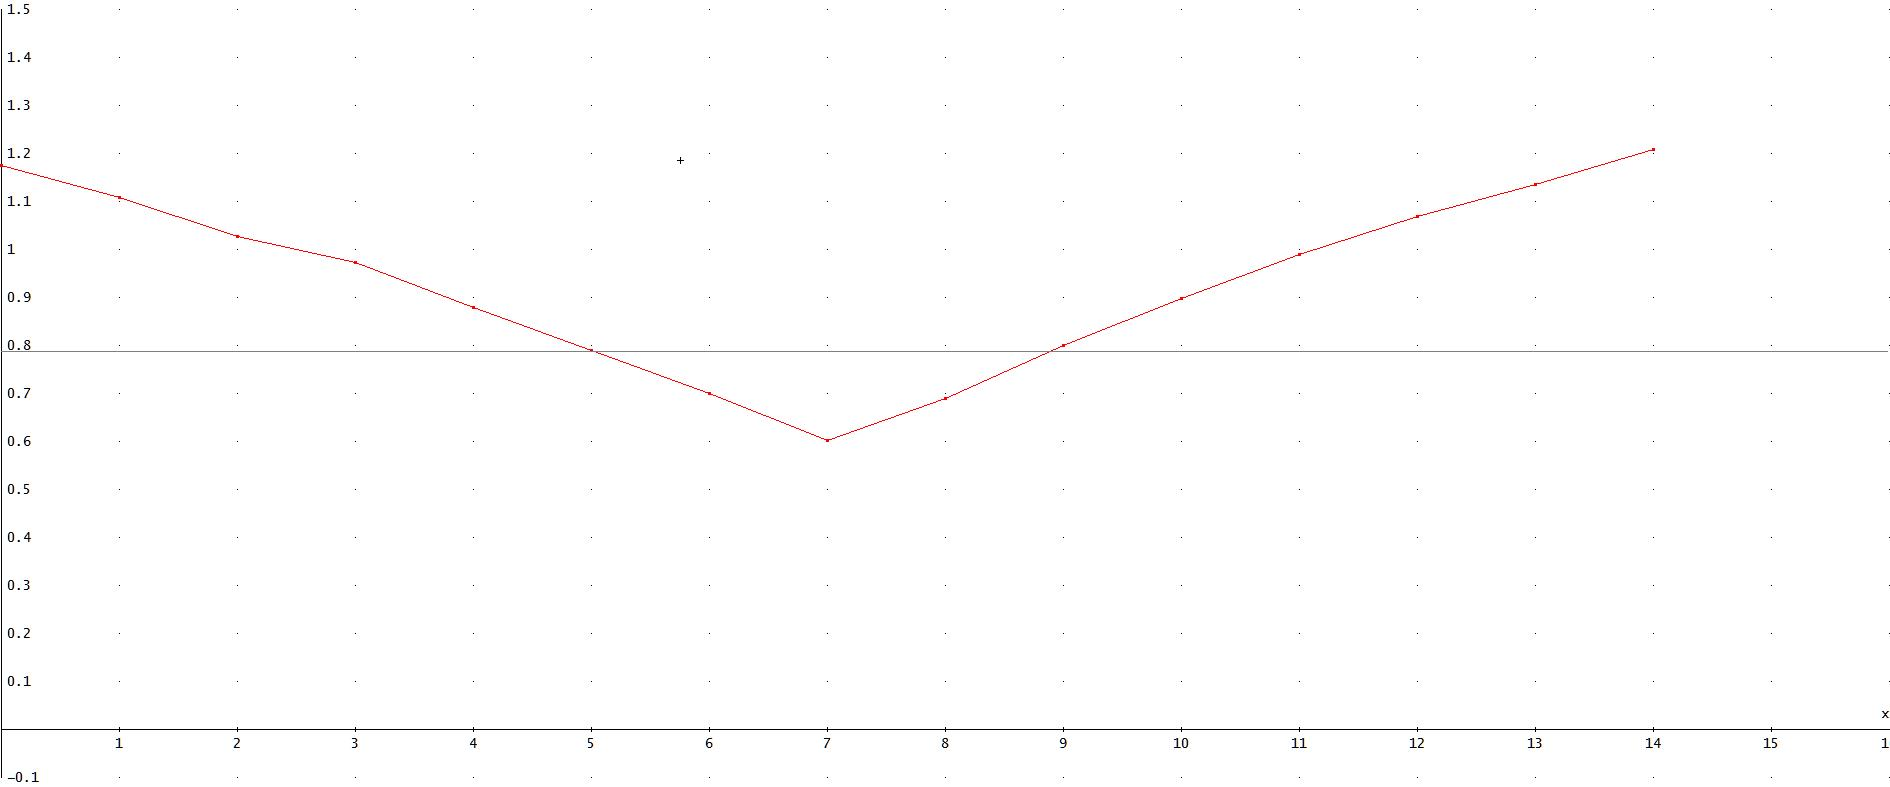
\includegraphics[width=0.95\textwidth]{Resources/result39-90-10.jpg}
	\caption{Squared l2 distances (y axis) of the subset of 39 morphs (with 15 steps on the x axis) compared to the corresponding compare photos, in contrast to the calculated threshold of 0,78666402} \todo{beschreibung anpassen}
	\label{fig:Result39-90-10}
\end{figure}